\chapter{Experiments}
\label{ch:experiments}

Every theoretical detail may look cool, but it has to show its worth in practice. In this chapter it is presented how experiments are conducted, from which the results are discussed further in chapter \ref{ch:res}. To start off, we narrow down our experimental research from the bag of ideas discussed in previous chapter in section \ref{sec:goal}. The metrics to objectively (which is crucial to retain an unbiased system) evaluate our models are shown in section \ref{sec:metrics}. Finally, section \ref{sec:expsetup} gives an overview of the total system with its design choices. Furthermore, all hyper-parameters are summarized. 

\section{Goal}
\label{sec:goal}
The holy grail is, as explained before, in this document the ability of machines to master the complete chess game through self play only, i.e. by gaining experience without a biased supervisor. This is however way too big for a master's thesis scope, which is why the constraint to relatively easy endgames was chosen. As we will see, this has the nice benefit it can be compared with optimal play. These models could be used to learn more complex chess positions as well from the bottom up.\\

A main difference between what we have discussed so far and other research is the use of bitboard features as input for a \gls{cnn}. In the end it would be interesting to study whether this is a promising idea.\\

The current state of the art \gls{td}-learning  algorithm for tactical board play is TD-Leaf($\lambda$). We compare this algorithm with the in section \ref{subsec:tdrootleaf} presented TD-Stem($\lambda$).

\section{Metrics}
\label{sec:metrics}
We show in this section how we can qualitatively assess and compare performances of learned models.

\subsection{Learning Curves}
\label{subsec:lc}
A typical plot used for assessment of \gls{rl} models is the learning curve. With these curves we can compare how fast agents are learning to optimize their rewards. The number of episodes $N$ are plotted against the running average of cumulative reward per episode $\mu_r$. These plots typically look similar to the plot in figure \ref{fig:psych}.\\
\begin{figure}
\centering
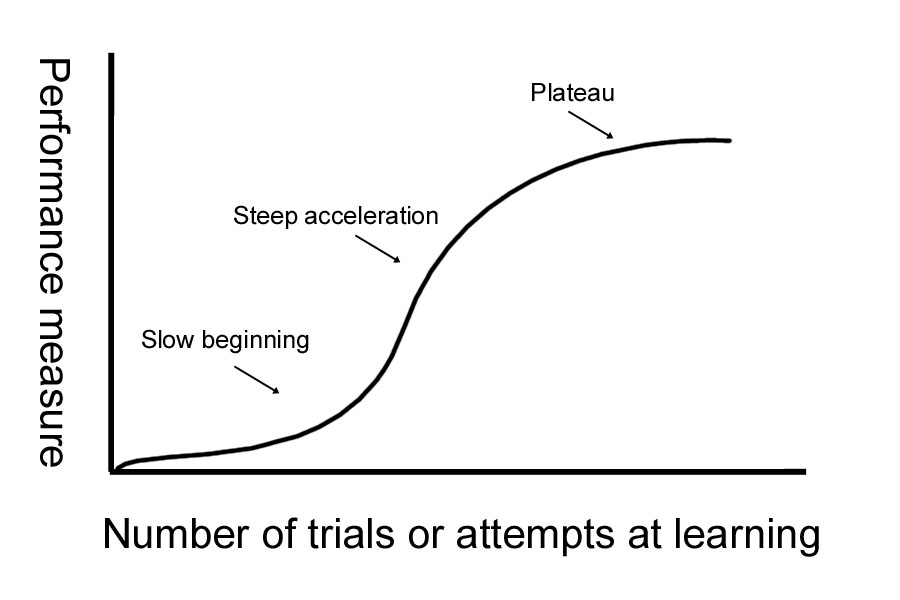
\includegraphics[]{fig/learning_curve}
\caption[learning curve]{The typical form of a learning curve, which looks like a logistic function. A slow start is followed by a steep acceleration in learning after which a plateau is reached. Interestingly, this image comes from a psychology book \cite{psych}.}
\label{fig:psych}
\end{figure}
In this thesis, some modifications of the classical learning curve with respect to the performance measure are used as alternatives. When we know for instance that most positions are a priori won, we can assess the performance of the model by checking the winning rate, which is
\[
Q_w=\frac{\text{number of games won}}{N}
\]
Like all averages, this can be tracked with a running averages.\\
Similarly, some positions should lead to checkmate faster and faster over the course of the learning process to prove that the agent learned to play more efficiently. Another performance measure is thus the average length. Formally, with $L_i$ the length of episode $i$, this measure is represented as follows:
\[
Q_l=\frac{1}{N}\sum_{i=0}^{N}L_i
\]

\subsection{Optimal Opponent Evaluation}
\label{subsec:opt}

Suppose for the sake of argument that we have an optimal player $O$, always making the right move. As an additional bonus, the final result is a priori known from the initial state $s$ of an episode $i$ taking optimal play from both players into account. We call this quantity the \gls{wdl}. From the perspective of a player $A$ 
\begin{equation*}
R_{wdl,A}(s)=\begin{cases} 
1 & \text{theoretical win } A \\
0 & \text{theoretical draw} \\
-1 & \text{theoretical loss } A\\
\end{cases}
\end{equation*}
If we were to have these optimal players, the \acrlong{dtm} is available as well. We call this quantity $L_{dtm}:\mathcal{S}\mapsto\mathbb{N}_{>=0}$ and it is the length of a game between optimal players.\\

Suppose we have designed a player $A$ using a model learned through self play on positions where we know the theoretical outcome and \gls{dtm}. If we let it play at its full strength some amount of games against an optimal player, we subsequently encounter N states with full a priori knowledge. By storing the statistics about every final result $R_A(s)$ and game length (in plies) $L_A(s)$ associated with the states, some useful strength indications of $A$ can be derived. To make notations easier:
\begin{align*}
W&=\left\{s|R_{wdl,A}(s)=1\right\} \\
W_A&=\left\{s|R_{A}(s)=1\right\} \\
D&=\left\{s|R_{wdl,A}(s)=0\right\} \\
D_A&=\left\{s|s\in D \wedge R_{A}(s)=0\right\}
\end{align*}

\begin{itemize}
\item The \textbf{\gls{wcr}} indicates how frequent the player is able to finish off a won position against a strong opponent.
\[
Q_{wcr,A}=\frac{|W_A|}{|W|}
\] 
\item With the \textbf{\gls{we}}, we learn how optimal the player converts the won position to checkmate.
\[
Q_{we,A}=\frac{1}{|W_A|}\sum_{s\in W_A}\frac{L_{dtm}(s)}{L_A(s)}
\]
It is easy to see how $0\leq Q_{we,A}\leq1$, as the optimal length of a won game is always smaller or equal than the actual observed length.
\item The \textbf{\gls{dcr}} is very similar to the \gls{wcr}, and quantifies the ability of $A$ to hold a draw against an optimal opponent.
\[
Q_{dcr,A}=\frac{|D_A|}{|D|}
\]
\item The \textbf{\gls{lhs}} is a signification of how strong $A$ defends lost positions. If the optimal player had to use the maximum of $L_{dtm}$ plies, $A$ behaved optimally.
\[
Q_{lhs,A}=\frac{1}{\left|(D \cup W)^c\right|}\sum_{s\in \left|(D \cup W)^c\right|}\frac{L_{A}(s)}{L_{dtm}(s)}
\]
Where $(D \cup W)^c$ is the complement of all drawn and won positions, hence, all lost positions. Equivalent to \gls{we}, $0<=Q_{lhs,A}\leq1$ and the equality with $1$ holds under optimal play from $A$. This measure is the fraction of the true game duration to the duration under optimal play.
\end{itemize}

With this bag of metrics, every game disregarding the theoretical result can be used to assess the quality of a model.\\

At first sight, these metrics may seem useless as chess has not been solved, and no 'optimal' player exists. However, recall the discussion in section \ref{subsec:tablebases} where we acknowledged the existence of tablebases yielding the exact information we need to use the performance measures defined here above for chess positions up to 7 pieces. Taking the gargantuan amount of storage into account for the 7 piece tablebase, we will restrict ourselves to 5 pieces. Although the size of this set of files is still 7 GB, it remains manageable. \\

These metrics are far from perfect, as they depend largely on the states provided. Some positions have much simpler paths to checkmate, and others are for example a certain draw where the player tested still goes for a win (which he would never achieve against a perfect opponent). We conclude this section by proclaiming the presented performance measure are more suitable for method comparison instead of real strength indicators.

\subsection{Value Curves}
\label{subsec:vc}
Considering the closer we get to mate, the better the position is for the winning side, we would expect the optimal value function $V^*(s)$ to be inversely proportional to the \gls{dtm}. From the winning player's perspective, he should always be able to improve his position. The player can only behave optimal with an $\alpha\beta$-search if the \gls{dtm} in the best leaf node (chosen upon the static evaluation) at the chosen depth of all states is indeed smaller than the root node. Hence, plotting the value function with respect to \gls{dtm} information is an indication of how much has been learned during self play.

\subsection{Speed}
\label{subsec:speed}
Due to the high complexity of the problem and its associated algorithms, a thoughtful implementation with respect to the computational cost is essential. The entire algorithm relies on two major components where speed can be measured in best interest: the move simulation in episodes and fitting the network to the data generated by this. The first will be measured in \gls{mps} while the latter is simply represented in seconds. Speedups are measured as the division of the duration in seconds of the old method by the duration of the new method.

\section{Experimental Setup}
\label{sec:expsetup}
With all that has been proposed yet, it is clear that this is not a trivial system to design, as there are lot of potential algorithms and hyper-parameters that can be tuned. It was necessary to fix a lot of these choices. As this is research, most solutions remain simple (Occam's razor \footnote{If there exist two explanations, the simpler one is usually better}), if someone were to continue research from here on, more complex systems can be designed.\\

Basically, it works as follows. A script with modifiable parameters is manually started. A fixed number of iterations are ran where the model is first playing against itself. When the model has played enough episodes and has gathered the necessary data, the learning algorithm is carried out onto the value network until the system starts to overfit.

This section contains an overview of a more detailed setup of the experiments.\\

\subsection{Search}
\label{subsec:search}
The search algorithm implemented is a combination of 2 $\alpha\beta$-pruning methods. First, an $\alpha\beta$-search without further optimizations is performed on the outcome of the game like in algorithm \ref{al:alphabeta_outcome}, looking for a forced win. If this indeed returns a forced win, the next stage is omitted. Else, a secondary search is required yielding the minimax evaluation with algorithm \ref{al:alphabeta} with two optimizations:
\begin{itemize}
\item the use of a transposition table. Although the speedup is minimal, it is consistent (1.03 \footnote{All speedups mentioned in this section were measured by playing 100 games with a value network as described in section \ref{subsec:exp_eval} and measuring the average time every method needed for calculating a move. Speedup is measured as $t_{old}/t_{new}$}), it was left in the main implementation of the search algorithm. The corresponding hash function is the default one of the programming language on a string representation of the chessboard. A transposition table with Zobrist hashing has been attempted well, but this proved to be less performant (speedup of 0.77, hence slower) \cite{patrascu12}.
\item stopping recursive calls when the depth left is equal to $1$. All possible states one ply ahead are fed immediately in one batch into the network to obtain the static evaluation. Vectorizing input speeds up de minimax evaluation, because most software libraries (like LAPACK) are optimized for that. Although less branches (with only one value left to calculate) are cut off the speedup is significant (2.24).
\end{itemize}
The first search can be performed at a higher depth than the second, because it is computationally some orders of magnitude less expensive for leave states to check whether the chess position is checkmate than to call the value network for an evaluation.

\begin{algorithm}
\caption{$\alpha \beta$-Result}
\label{al:alphabeta_outcome}
\begin{algorithmic}[]
\REQUIRE board, depth, $\alpha$, $\beta$
\ENSURE $\alpha$\\
\IF {board is checkmate}
\RETURN -1
\ELSIF{depthLeft $\leftarrow 0$}
\RETURN 0 
\ELSE
\FOR{move \textbf{in} \textit{LegalMoves}(board)}
\STATE newboard $\leftarrow doMove$(board, move)
\STATE score $\leftarrow -\frac{\alpha \beta Result(\text{newboard, depthLeft} - 1,-\beta,-\alpha)}{2}$
\COMMENT{faster mates are better}
\IF{score $\geq \beta$}
\RETURN $\beta$
%\COMMENT{$\beta$-cutoff}
\ENDIF
\IF{score $> \alpha$}
\STATE{$\alpha \leftarrow$ score}
%\COMMENT{$\alpha$ is the max from \textit{Minimax (Algorithm \ref{al:minimax})}}
\ENDIF
\ENDFOR
\ENDIF
%\ENDFOR
%\ENDIF
\end{algorithmic}
\end{algorithm}


\subsection{Evaluation}
\label{subsec:exp_eval}

\subsubsection*{Feature Space}
The input of our vectorization function in the experiments is a string representation of the board, named \gls{epd}. From this the bitboards are extracted like described in figure \ref{fig:feat} are extracted.The only global features that were added are the side to move, whether the position is a draw and whether it is mate. It follows that our feature vector consists out of $1539$ binary elements. Undoubtedly, better state representations using more bitboards and global features are possible  as presented in section \ref{sec:fs}, but the vectorization function proved to be a performance bottleneck. To be able to carry out more simulations the decision was taken to restrict to this basis input vector, considering it already contains almost all game play information.\\

Simulations have been executed on chess problems with a limited set of possible pieces on the board like the \gls{krk} and \gls{kqk} end games depicted in \ref{fig:subprob}. These require less channels as the state is less condensed with pieces. 

\begin{figure}
    \centering
    \begin{subfigure}[b]{0.4\textwidth}
        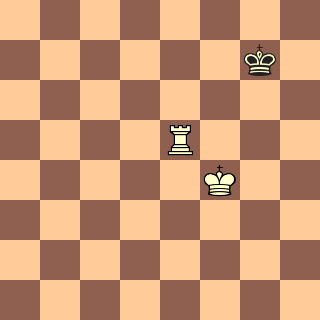
\includegraphics[scale=0.5]{fig/krk}
        \caption{\gls{krk} endgame}
        \label{fig:krk}
    \end{subfigure}
    \qquad
    \begin{subfigure}[b]{0.4\textwidth}
         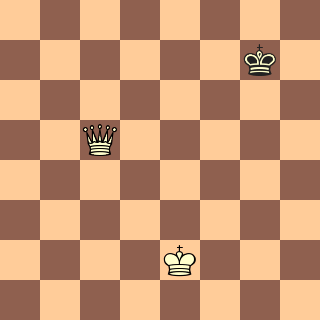
\includegraphics[scale=0.5]{fig/kqk}
        \caption{\gls{kqk} endgame}
        \label{fig:kqk}
    \end{subfigure}
    \caption[End games]{Subproblems where only two kinds of pieces are used. The dimension size of the input reduces to 515.}
    \label{fig:subprob}
\end{figure}

\subsubsection*{Network architecture}
There has been experimented with different \gls{cnn} architectures using the bitboards as input. The activation function between all hidden units is an ordinary \gls{relu} and the weights are initialized with the tips given by Bengio et al. \cite{init}.\\

\subsection{Self Play}
\label{subsec:selfplay}

The self play framework we employ is one with multiple agents, both black and white try to maximize their rewards. We have not experimented with the systems using one learning agent playing with the most up to date model against an older model \cite{alphago16,dddqn15}. The reason it has not been tested is the additional implementation cost to address two networks, hence two GPUs, in combination with time constraints.\\

In self play, episodes are set up and the model plays them up to a certain point. During self play, data is collected. This data is then used after some amount of episodes so it can be used to update the value network.

\subsubsection*{Setup episode}
Initial positions can be generated by random placing the pieces on the board and achieving a legal position. However, This method becomes more complex when more pieces need to be placed on the board. This is why in most experiments, in light of future research, the starting state is generated through a large dataset containing computer games \cite{dataset}. The large amount of \gls{epd}s that were generated through this were subsequently filtered according to the problems looked for. For example, an additional dataset only containing \gls{krk} positions was generated to solve the \gls{krk} problem.  It is made sure that all positions in the dataset are unique. There are still two main issues with naively random sampling positions and using them as initial state:
\begin{enumerate}
\item Due to the fact all positions originate from games, they are all part of a sequence. States from identical games are correlated to each other, especially when they are only a few moves away. This correlation may induce overfitting in the learning process.
\item We cannot validate our positions with the exact same dataset, as this would not prove that the learned approximation is an acceptable generalization.
\end{enumerate}
These problems are mitigated by making random moves before self play. An increasing amount of random moves decorrelates the input. However, the position may evolve too much by capturing pieces and pushing pawns. There was not enough time to limit the random moves to non captures and non pawn moves.\\

Aside from this additional randomization, we might split our datasets in a training, used for self play, and validation set to solve the second shortcoming.\\

\subsubsection*{Policy}
The policy of the agents during simulation has been restricted to $\epsilon$-greedy. As noted in section \ref{subsec:clil}, this works fine and for the scope of this thesis, and it is not necessary to try more elaborated policies. To try to speed up training though, there has been some examinations of decay functions. Two different decay functions are deployed, suppose $i$ is a integer linearly proportional to the number of simulated episodes, and f is an additional parameter:
\begin{enumerate}
\item Linearly adjusting the decay: $\epsilon_i\leftarrow1-fi$
\item To adjust for a slow start, we can begin by using a power $0.5<f<1$ to reduce $\epsilon$ with hyperbolic decay: $\epsilon_i\leftarrow\frac{1}{(i+1)^f}$
\end{enumerate}

The greedy action is taken in the direction of the minimax search described in \ref{subsec:search}, as in classical engines. This is the same for both examined TD($\lambda$) algorithms. The depth of search is for our purposes limited to 3, to guarantee fast simulations.

\subsubsection*{Episode Termination}
The game is continued until a terminal state i reached, or a maximum number of actions has been performed, after which the game and its data are stored in replay history and a new episode is generated in the same fashion.

\subsubsection*{Self Play Termination}
An iteration of self play goes on until enough games have been recorded with notable rewards (i.e. episodes ending with checkmate). The rationale behind this is that at first, most games end undecided (because random play increases the probability of exceeding the maximum number of allowed moves).

\subsubsection*{Learning Algorithm}
When a self play iteration has been completed, we perform the following steps to improve our network with mini-batch \gls{sgd}:
\begin{enumerate}
\item \textbf{Data assimilation.} This phase is simply collecting all episodical data (featurized states and rewards). Every episode has to be examined in detail independently in the following steps.
\item \textbf{Calculation target values.} The $\lambda$-returns are calculated with TD-Stem($\lambda$) or TD-Leaf($\lambda$). The discount rate is fixed to $\gamma=1$, but the implementation is flexible enough to handle other values. In this manner, TD-Leaf($\lambda$) as implemented in the system is equivalent to previous research.
\item \textbf{mini-batch \gls{sgd}.} At the end of every iteration, the network gets an update with mini-batch \gls{sgd}.
\end{enumerate}

Furthermore, we have added some optimizations to this process based on observations when testing the implementation:
\begin{itemize}
\item When learning has just started and the agent is mostly in an exploring mood, only the last values of the episodes are kept, as the start of the episode is mostly noise. By throwing this noise away, we accelerate initial training.
\item Memory problems show up (a very bad performance) when keeping all returns. Hence, it is ensured that training data does not exceed a maximum size (50000 samples). At the same time, every episode has the same contribution to this dataset. The training samples used for supervised learning later in the process are moved to a buffer object, also storing tuples from previous value network update iterations, to decorrelate the samples and thus reduce overfitting.
\item The data to update the network is picked randomly from the buffer object. Samples recorded during more recent play have a higher probability of being picked. Depending on the network, a different learning rate is used. Deeper networks have the tendency of needing a smaller learning rate.
\end{itemize}

\subsubsection*{Experimental Methodology}
By running a script, the system is set up. An initialized value network learned from a previous run can be given as a parameter. These runs are ad hoc, and the decision for the parameters can change in between runs. This way of working increases the flexibility of adjustments. Every separate run from a script will be called a stage from now on. It speaks for itself that stages with the same parameters must be ran to obtain useful comparisons. The parameters that were adjusted in between the stages are laid out in table \ref{tab:params_exp}. \\

In general, the exponential weight decay parameter $\lambda$ from TD learning increases over the stages, because the more training evolves, the higher our confidence in assigning credit to moves further away from checkmate. Similarly, the number of moves used to calculate the $\lambda$-return increases along the script. It also makes more sense to start off with a small depth, and increase it along the way for a faster decent initialization of the network. Starting off with deep searches seems like overkill and a waste of computation power.

\begin{table}[]
\centering
\caption{Hyper-parameters modifiable in between stages.}
\label{tab:params_exp}
\begin{tabular}{rl}
 \hline
$\lambda$    & trace decay parameter for TD-learning methods                                                                                                        \\ 
$d_r$        & Depth at which final results are examined in search                                                                                      \\ 
$d_V$        & Depth at which the value network is called                                                                                               \\ 
$f_\epsilon$ & \begin{tabular}[c]{@{}l@{}}Decay function for exploration parameter $\epsilon =f(i)$.\\  i increments every iteration.\end{tabular}      \\ 
$I$          & Number of iterations                                                                                                                     \\ 
$i_0$        & First iteration number, to initialize $\epsilon$ with the $f_\epsilon$                                                                   \\ 
$K$          & \begin{tabular}[c]{@{}l@{}}The number of states that are used to calculate the $\lambda$-return \\ from an episode\end{tabular}          \\ 
$M$          & The maximal amount of moves made in an episode                                                                                           \\ 
$N$          & How many games are played during an iteration                                                                                            \\ 
$R$          & \begin{tabular}[c]{@{}l@{}}The number of additional random moves played on the board position \\ extracted from the dataset\end{tabular} \\ \hline
\end{tabular}
\end{table} 

\subsection{Implementation}
\label{subsec:software}
All experiments were carried out on GPU servers. To be specific everything was tested on either a NVIDIA GeForce GTX 680 4GB with an Intel(R) Core(TM) i7 CPU 930 @2.80GHz (6 CPUs) or NVIDIA Tesla K40c 12GB with an Intel(R) Core(TM) i7-3930K CPU @ 3.20GHz. We will call the former machine A and the latter machine B.\\

All code is written in Python v2.7, with a chess engine written in C. At first, all chess specific knowledge was extracted through the Python chess library, but it became clear that performance could be enhanced enormously by using native C code (the Python chess library is still used at some parts, but rarely) \cite{pychess}. The neural networks are implemented with Tensorflow, an open source software library for machine intelligence.\\

All implementations were serialized at first, but the necessity to parallelize the code is obvious. A speedup almost linear proportional to the number of CPUs in the machine is achieved by concurrently simulating the episodes.  Quite some work was put into the synchronization of all components with the Python multiprocessing module, as the network has to calculate values for all episodes. After playing $N$ episodes, the network has to be called again, now to fit to the data.\\
A high level architecture of the written software \footnote{open source \cite{rookie}} is shown in figure \ref{fig:arch}. The \textit{supervisor} is created in a main process (there can only be as many processes as CPUs in the Python design) and controls all work. Before simulating episodes the supervisor creates a new process responsible for the value network, whose calculations are performed on the GPU. thereafter the following steps are executed iteratively:
\begin{enumerate}
\item The supervisor creates as many processes as there are CPUs available and commands them to perform $N$ episodes in total. Next, the supervisor goes to sleep and waits until these jobs are finished.
\item The agents need to call the value network, but the GPU resource can only be taken once at a time, which is why all requests are stalled in a FIFO queue if necessary
\item Whenever an episode terminates, it dumps its recorded data in a buffer. As all episodical processes are trying to drop data, this is handled in a queue as well.
\item When all $N$ episodes have terminated, the supervisor wakes up and passes data from the buffer to the value network again with the purpose to improve the value function with \gls{sgd}.
\item After fitting, these steps repeat themselves until the desired convergence has been attained.
\end{enumerate}

\begin{figure}
\centering
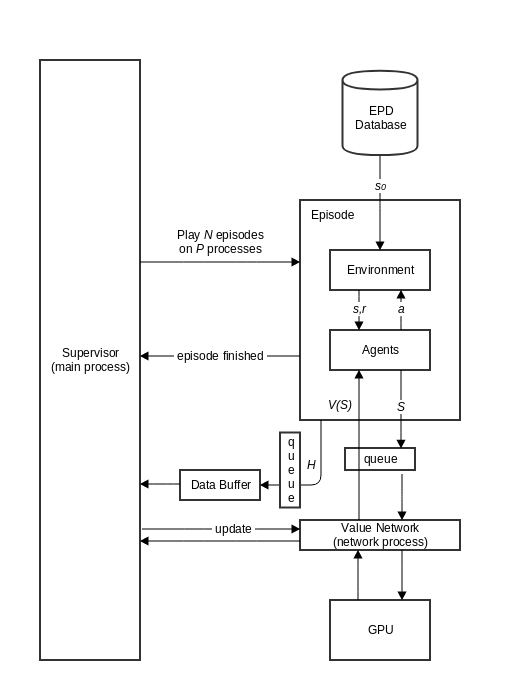
\includegraphics[scale=0.8]{fig/flow}
\caption{High level software architecture of the simulation system.}
\label{fig:arch}
\end{figure}